\RequirePackage{amsmath}


\DeclareMathOperator*{\argmax}{arg\,max}
\DeclareMathOperator*{\argmin}{arg\,min}
\newcommand{\R}{\mathbb{R}}


\documentclass{article}

\usepackage[numbers, sort&compress]{natbib}
% \usepackage{pdfpages}
\usepackage{rotating}
\usepackage{amssymb}
\usepackage[margin=1in]{geometry}
\usepackage{graphicx}
\usepackage[strings]{underscore}
\usepackage{anyfontsize}
\usepackage{subcaption}
% \usepackage{lipsum}
\usepackage[toc]{appendix}
% \usepackage[utf8]{inputenc}

\begin{document}


\title{Deep-learning emulators of transient compartment fire simulations for room-scale calorimetry}




\author{}
\date{March 18, 2020} 

\maketitle

\begin{abstract}

\end{abstract}
\section{Introduction}
Compartment fire models are useful for many applications. For one, accurate predictions of potential fire scenarios help quantify the risk of adverse consequences such as property damage and loss of life. They also can provide insight in forensics problems by identifying fire credible fire scenarios given the observed evidence. The value of accurate models is also augmented by the fact that compartment fire experiments are difficult and expensive to perform. 

The computational expense of fire simulation tools varies significantly. For instance,  ``zone" models typically run at super-real-time speeds because of their relatively simple physics. These models are useful for probabilistic assessments \cite{anderson2018quantifying, baker2013developing} and other applications that require results from many simulations. Zone models typically divide a compartment into two homogeneous zones- an upper gas layer of hot combustion products, and a cooler lower layer. Examples of commonly used zone models include the Consolidated Model of Fire and Smoke Transport (CFAST) \cite{peacock1993cfast} and BRANZFIRE \cite{wade2000branzfire}. Conversely, computational fluid dynamics (CFD) models are significantly more computationally expensive, but are generally more accurate. These models are also capable of making predictions for specific locations in the compartment, rather than for large spatially averaged zones. 

There have been various efforts to combine the advantages of CFD and zone models. Hostikka et al. \cite{hostikka2005two} proposed a Two-model Monte Carlo approach that uses a relatively small number of FDS runs to correct the results from a larger number of CFAST runs to produce a probabilistic output. Outside of compartment fire modelling, there are many studies that have explored the coupling of zone models with CFD models for various applications \cite{dreng2008method, tan2005application, wang2007validation, colella2009calculation, floyd2011coupling, colella2011multiscale}. 

The recent advances in machine learning have allowed for novel methods of producing models that combine the accuracy of CFD models with the computational speed of zone models. Hodges et al. \cite{hodges2019compartment} and  Lattimer et al. \cite{lattimer2020using} have proposed using transpose convolutional neural networks (TCNNs) for producing spatially resolved temperature and velocity fields for steady compartment fires. Although the present work is similar to these studies in the sense that deep learning is leveraged to develop "emulators" of FDS, there are several key differences. First, rather than predicting the full temperature field in a steady compartment fire, the aim of the present study is to predict the transient temperature evolutions at specified location for a compartment fire with a transient heat release rate evolution. These locations correspond to the locations of thermocouples in an experimental configuration. Another key difference is the role of zone models in the methodology. Rather than using zone model results as inputs to the deep learning models, they are used for \textit{transfer learning} \cite{pan2009survey}. This is a concept heavily used in Natural Language Processing (NLP) \cite{ruder2019transfer} and computer vision \cite{gopalakrishnan2017deep} applications. The idea is that an agent can learn a new task more efficiently if it has already been trained to perform a similar task. In the present study, the artificial neural networks (ANNs) are first trained to produce outputs from a zone model, with which a large training set can be obtained easily. These ANNs are then trained to produce FDS results. The result is that the pretrained ANNs can learn to produce accurate FDS results with much fewer FDS runs than non-pretrained ANNs. An advantage of this approach is that when the model makes predictions for a new case, the zone model does not need to be run again, which would be a speed-limiting step. 

This paper also explores the utility of using FDS emulators for inverse problems. These problems involve using observations to infer the causal factors that produced them. Essentially the goal is to run FDS in reverse; from a set of simulation outputs, the goal is to determine the simulation inputs that produced them. This cannot be done directly in FDS, so iterative techniques requiring many runs for a single scenario are often required, which is especially computationally expensive. Deep learning can aid this process not only by reducing the time it takes to produce FDS results, but also by obviating the need for iteration altogether. This is because ANNs can be trained to map FDS outputs to FDS inputs directly, which makes the inversion process even faster. 

The specific inversion problem explored in this paper is to determine a fire's transient heat release rate (HRR) from a series of transient thermocouple measurements. The HRR has been described as the most important variable in fire hazard assessment \cite{babrauskas1992heat}. It describes the amount of energy that is released from the combustion reactions of a fire, and it is a predictor for the onset of adverse fire consequences such as flashover \cite{mccaffrey1981estimating} and secondary ignition \cite{jahn2008effect}. Many methods exist to measure HRR at various scales. Perhaps the most common calorimetry apparatus at the bench scale is the cone calorimeter \cite{babrauskas1984development} developed by Babrauskas at NIST. This approach is based on measuring the oxygen consumed during the fire. Because the heat of combustion per unit of oxygen consumed is approximately constant across most fuels encountered in fires \cite{huggett1980estimation}, the oxygen consumption measurements can be easily converted to estimates of the heat release rate. Another apparatus is the OSU calorimeter \cite{smith1996heat}. Unlike oxygen consumption calorimeters, this apparatus measures temperatures at various locations that allow for the HRR to be estimated by a simple energy balance. 

Full scale calorimetry measurements are more difficult to obtain. Open burning calorimeters have been developed to measure the HRR of furniture items \cite{babrauskas1982upholstered}. However, a limitation of these approaches is that the burning conditions do not necessarily resemble those of an actual compartment fire. To account for room effects, oxygen depletion calorimetery has been applied to room-scale fire tests \cite{abecassis2008characterisation}. These measurements are often expensive and difficult to set up, which has led to an effort to develop more cost effective full scale HRR inversion frameworks. Most of these approaches rely on using correlations or two-zone models to invert for the HRR. Richards et al. \cite{richards1997fire} used temperature data from ceiling sensors to estiamte the HRR using LAVENT, a two-zone model. Overholt and Ezekoye \cite{overholt2012characterizing} developed a inversion framework that uses measurements of the upper gas layer temperature with the zone-model CFAST. Kurzawski and Ezekoye also developed a methodology using heat flux measurments from Directional Flame Thermometers (DFTs) with the FDS as the forward model. The present work is a natural extension of these studies in that it utilizes temperature measurements with the physics of FDS for HRR inversion.

\section{Experimental setup}
An experimental compartment measuring 5~m by 6~m by 2.4~m previously utilized for various room scale fire experiments including positive pressure ventilation~\cite{Weinschenk:2011}, wildfire fuel bed characterization~\cite{Overholt:2014}, and HRR inversion~\cite{Kurzawski:2017} at the J.J. Pickle Research Campus at the University of Texas at Austin was used to conduct further testing for HRR inversion experiments. All interior walls are lined with 1.6 cm gypsum wallboard and the floor is 2.54 cm thick and made of concrete. 
For the burner experiments, one sand burner 0.3~m by 0.3~m square with a height of 0.4~m constructed in accordance with the standard \textit{NFPA 286} was electronically controlled using an Alicat Scientific MCR-series 250 SLPM PID mass flow controllers to follow specified HRRs~\cite{NFPA:286}. The sand burner was placed in the center of the compartment. A National Instruments data acquisition system was used to send setpoint signals to the Alicat mass flow controllers to control the flow of propane to the burner within the compartment. The data rate for all experiments was set to 1~Hz. Four burner experiments were conducted, each with a different prespecified HRR ramp. These included two triangle fires- one with a 300 second time to peak and one with a 100 second time to peak, a symmetric t-squared fire, and an arbitrary ramp that was chosen to resemble the potential behavior of an actual burning item whose HRR may grow and diminish unpredictably throughout an experiment. The four HRR ramps are shown in  

\begin{figure}[htb] \centering
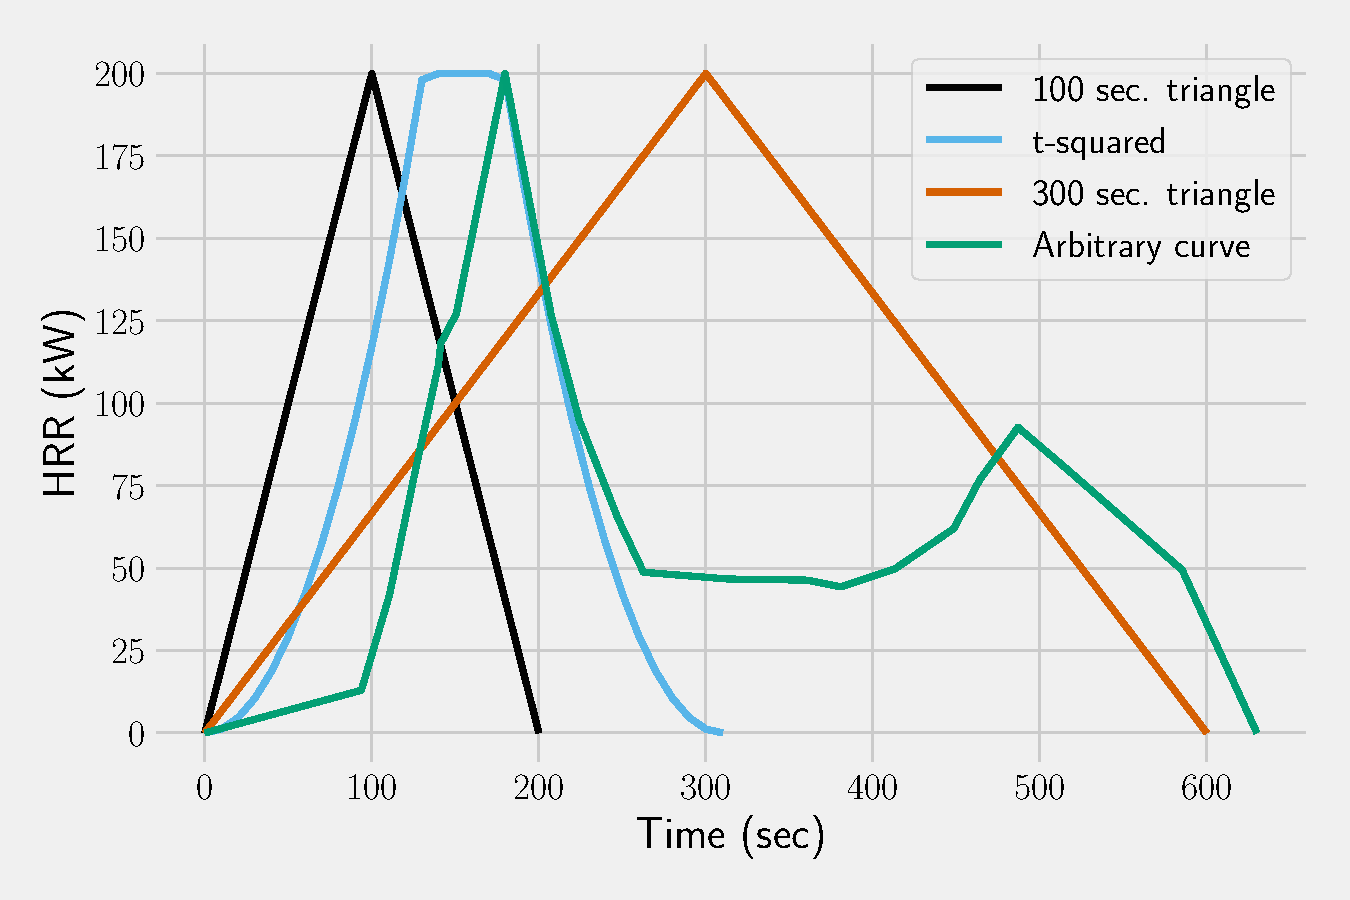
\includegraphics[width=.75\textwidth]{figures/training_ramps.pdf}
\caption{The four specified HRR ramps for the burner experiments.}
\label{fig:burner_ramps}
    \end{figure}


\begin{figure}[htbp]
  \centering
  \begin{subfigure}[t]{.301\textwidth}
      \centering
      \includegraphics[width=\textwidth,keepaspectratio]{figures/burner.pdf}
      \caption{Propane burner fire}
      \label{fig:fire_image}
  \end{subfigure}
  \begin{subfigure}[t]{.3\textwidth}
      \centering
      \includegraphics[width=\textwidth ,keepaspectratio]{figures/nhexane.pdf}
      \caption{N-hexane pool fire}
      \label{fig:brightness_heatmap}
  \end{subfigure}
  \begin{subfigure}[t]{.3\textwidth}
      \centering
      \includegraphics[width=\textwidth ,keepaspectratio]{figures/methanol.pdf}
      \caption{Methanol pool fire}
      \label{fig:binary_fire_image}
  \end{subfigure}
  \caption{Photos from each of the three types of fire experiments conducted for this study.}
\end{figure}
\section{Computational models}
Two computational models of the experimental setup were used in this study- one in CFAST and one in FDS. The CFAST model serves only for pretraining the ANNs that eventually learn to emulate FDS. 
\subsection{Consolidated Model of Fire and Smoke Transport (CFAST)}
Because the CFAST model is only used for transfer learning, it is a relatively simple description of the experimental setup. 


\subsection{Fire Dynamics Simulator (FDS)}
\section{Emulators of FDS with ANNs}
\subsection{Building the training set}
A key step developing the emulators is to determine a viable strategy for building the training set. This involves generating randomly draws for the HRR curves, but an appropriate construction of the random draws is not straightforward. One may think to specify the functional form of the HRR curve (i.e. t-squared or triangle ramps) and randomly draw the corresponding parameters. This approach is limiting because the ANNs then likely would only be able to produce reliable results for these \textit{parametric} HRR curves. Instead, a non-parametric description of the HRR curvies is preferred. This means that an HRR curve is drawn without specifying a functional form. There are also potential issues with this approach; if one draws independent random values at different times to construct the HRR curve, then that would produce unphyisically ``noisy" HRR curves.

The Gaussian process formalism allows for the development of a generative model that circumvents these issues. A Gaussian process is a stochastic process in which any finite collection of random variables has a joint multivariate normal distribution \cite{lee2017deep}. This concept can be a bit abstruse for those unfamiliar with this type of statistical modelling, so a more in-depth explanation is provided here. The overall goal is to describe a probability distribution of reasonably smooth functions. If this distribution exists, then one could draw a random sample of $N$ functions, i.e. $f_n(t), n \in \{1,2,.., N\}$, where each $f_n(t)$ is a randomly drawn function defined over $t$. At any specified time, $t'$, one could evaluate every drawn function at $t'$.  This would result in a sample of size $N$ of scalar function evaluations, $f_n(t')$. According to the definition of a Gaussian process, $f_n(t')$ is normally distributed for any $t'$. Now, one could imagine evaluating each of the functions at \textit{two} points, $t_1$ and $t_2$, resulting in two scalar function evaluations for each $f_n(t)$. Again, if the distribution of functions is a Gaussian process, then the vectors $[f_n(t_1), f_n(t_2)]^T$ will have a bivariate normal distribution. Similarly, for any size $k$ vector of times, $\boldsymbol{t} \in \R^k$, $f(\boldsymbol{t})$ is $k$-variate normally distributed. The general equation for a multivariate normal distribution is shown in equation \ref{eqn:multivariate_gaussian}.

 \begin{equation}
  \label{eqn:multivariate_gaussian}
  p\bigg(f(\boldsymbol{t}) \bigg) =
  (2\pi)^{-\frac{k}{2}}\text{det}\big[\boldsymbol{\Sigma}\big]^{-\frac{1}{2}}\text{exp}\bigg(-\frac{1}{2}\big[f(\boldsymbol{t}) - \boldsymbol{\mu}\big]^T \boldsymbol{\Sigma}^{-1}\big[f(\boldsymbol{t}) - \boldsymbol{\mu}\big] \bigg)
\end{equation}



\noindent Just as a univariate normal distribution is uniquely characterized by a scalar mean and a scalar variance, a multivariate normal distribution is uniquely characterized by a mean \textit{vector}, $\boldsymbol{\mu}$  and a covariance \textit{matrix}, $\boldsymbol{\Sigma}$, which must be symmetric and positive semi-definite. The entries of $\boldsymbol{\Sigma}$ are described in equation \ref{eqn:covariance_matrix}.

 \begin{equation}
  \label{eqn:covariance_matrix}
  \Sigma_{i,j} = E\bigg([x_i- \mu_i][x_j - \mu_j] \bigg)
\end{equation}

\noindent where $E$ is the expectation operator, $E(x) =  \int_{-\infty}^{\infty} xp(x) dx$. The diagonal terms of  $\boldsymbol{\Sigma}$ describe the variance of the corresponding function evaluations. The off-diagonal terms describe the correlation between two function evaluations. To make this more clear, the bi-variate example is revisited. If $\boldsymbol{t} = [t_1, t_2]^T$, and $t_1 = t_2$, then obviously $f_n(t_1) = f_n(t_2)$ for any randomly drawn continuous function $f_n(t_1)$. Said differently, $f_n(t_1)$ and $f_n(t_2)$ are perfectly correlated. If instead, $t_2 = t_1 + \Delta t$, then there is no guarantee that $f_n(t_1) = f_n(t_2)$, but it is reasonable to expect that $f_n(t_1)$ and $f_n(t_2)$ are correlated if $\Delta t$ is small. If $\Delta t$ is large, then one would expect that $f_n(t_1)$ and $f_n(t_2)$ are uncorrelated. Figure \ref{fig:gp_illustration} provides an illustration of the idea of covariance between function evaluations. 

\begin{figure}[htbp]
  \centering
  \begin{subfigure}[t]{.45\textwidth}
      \centering
      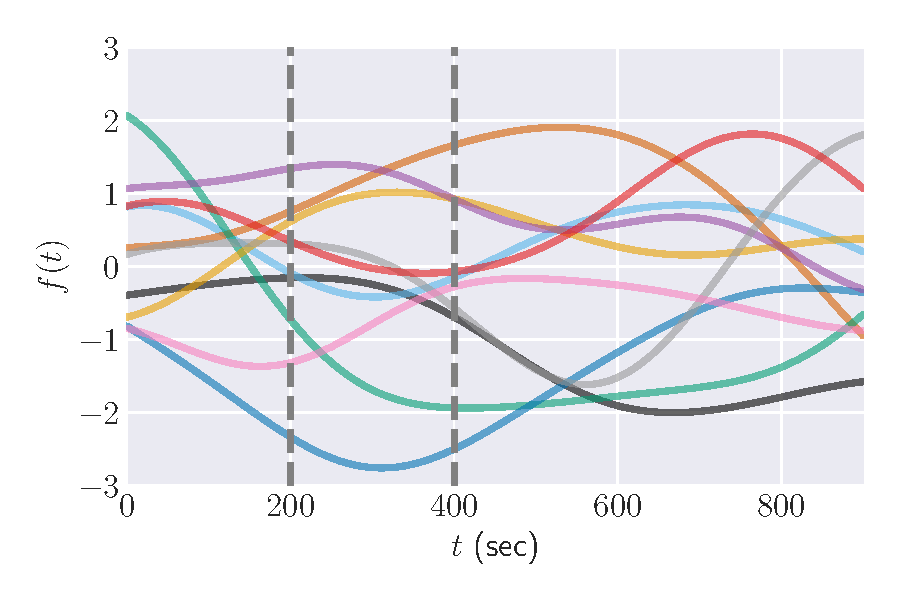
\includegraphics[width=\textwidth,keepaspectratio]{figures/gp_draws.pdf}
      \caption{Random draws from an arbitrary GP}
      \label{fig:gp_draws}
  \end{subfigure}
  \begin{subfigure}[t]{.45\textwidth}
      \centering
      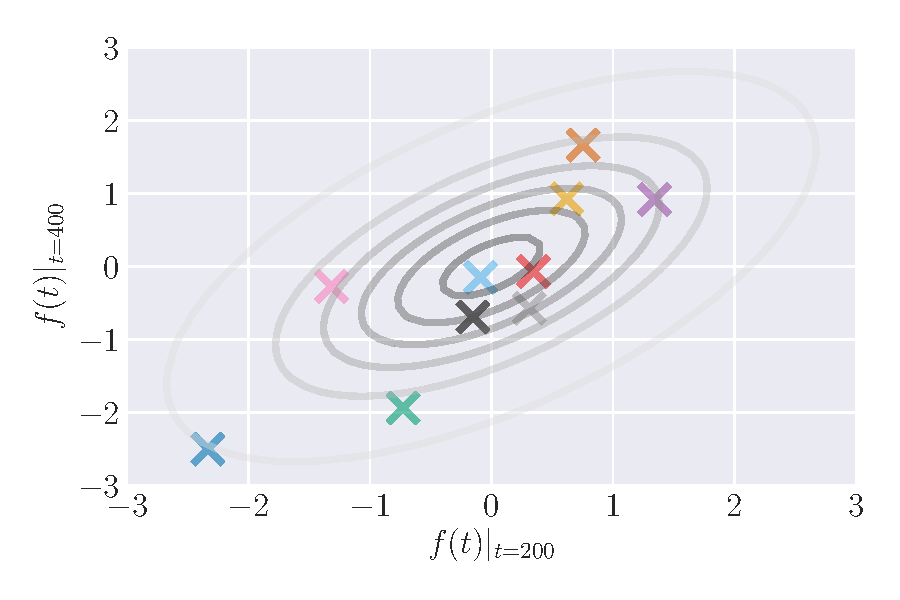
\includegraphics[width=\textwidth ,keepaspectratio]{figures/gp_scatter.pdf}
      \caption{Scatterplot of function evaluations with bivariate PDF}
      \label{fig:gp_scatter}
  \end{subfigure}
  \caption{\protect\ref{fig:gp_draws} shows 10 randomly drawn functions from an arbitrary Gaussian process. Each randomly drawn function is evaluated at $t=200$ seconds and at $t=400$ seconds. A scatterplot of these function evaluations is shown in \protect\ref{fig:gp_scatter}. Note that the function evaluations at the two different times are correlated. Also, the defining characteristic of a Gaussian process is that these quantities must be normally distributed, so the contours of the bivariate probability density function are also shown. If this process were repeated for many more randomly drawn functions, the contours would indicate the density of points.}
  \label{fig:gp_illustration}
\end{figure}


Just as a multivariate normal distribution is uniquely characterized by a mean vector and a covariance matrix, a Gaussian process is uniquely characterized by a mean \textit{function}, $m(t)$ and a covariance \textit{function}, $K(t_i, t_j)$. Then for any vector of times $\boldsymbol{t}$, the resulting multivariate normal distribution can be characterized computing the mean vector $m(\boldsymbol{t})$ and the covariance matrix $K(\boldsymbol{t}, \boldsymbol{t})$. Based on the intuition that the degree of correlation between $f_n(t_i)$ and $f_n(t_j)$ should depend on the magnitude of $\Delta t = t_i - t_j$, the squared exponential kernel is a common choice for a covariance function. Its form is shown in equation \ref{eqn:squared_exponential}, 

 \begin{equation}
  \label{eqn:squared_exponential}
    K(t_i, t_j) = \tau^2exp\bigg(-\frac{(t_i-t_j)^2}{2b^2}\bigg)
\end{equation}

\noindent where $\tau^2$ is a hyperparameter that describes the magnitude of the function draws, and $b$, known as the bandwidth, relates to the time scale over which function evaluations are correlated. Intuitively, $b$ defines how smooth the function draws will be, with a larger bandwidth giving smoother functions. This covariance function has a ``bell" shape; it reaches a maximum as $t_i - t_j$ approaches zero and asymptotically approaches zero as $t_i - t_j$ goes to positive infinity or negative infinity. 

For generating the training set of the FDS emulators, an initial Gaussian process is specified for the transient HRR, i.e. $\dot{Q}(t)\sim \mathcal{GP}\bigg(m_0(t),K_0(t_i,t_j)\bigg)$, with $m_0(t)=$ 150 kW, meaning at at any time, the function evaluations will be centered around 150 kW. The covariance function, $K_0(t_i,t_j)$ is specified according to equation \ref{eqn:squared_exponential}. The hyperparameter, $\tau^2$ is chosen to be 8,100 kW$^{\text{2}}$, meaning that the standard deviation of any individual function evaluation is $\sqrt{8100} = 90$ kW, producing a reasonable variation of HRR values centered around 150 kW. Two bandwidth values, $b$,  were used. In about half of the draws, the bandwidth was set to 30 seconds and in the other half, the bandwidth was set to 60 seconds. This was done so that the training set would contain both smooth and more rapidly changing HRR curves. 


To draw HRR curves for the ANN training set, a time vector $\boldsymbol{t}^{\text{NN}} = [0, 10, ..., 900]^T$ was specified. This vector contains 91 evenly spaced points between 0 and 900 seconds (inclusive). 900 seconds (15 minutes) was chosen because it is the maximum simulation duration for the cases of interest in this paper. For other applications, this vector could be specified differently to allow longer simulations. Evaluations of randomly generated functions can then be generated by specifying a multivariate normal distribution with mean $m_0(\boldsymbol{t}^{\text{NN}})$ and covariance $K_0(\boldsymbol{t}^{\text{NN}},\boldsymbol{t}^{\text{NN}})$. The Python package Scipy \cite{jones2001scipy} was used for performing the random multivariate normal draws. 

The astute reader may notice that these multivariate normal draws still do not necessarily produce viable HRR curves. The HRR should be zero at the point of ignition, i.e. $\dot{Q}(0) = 0$. Also, at the end of the simulation, the HRR should ramp back to zero, i.e. $\dot{Q}(t_{end}) = 0$, where $t_{end}$ is the duration of the fire. It is desired that the emulators can produce FDS outputs of simulations with varying $t_{end}$. As a result, $t_{end}$ is uniformly drawn between 150 and 900 seconds for each case in the training set. Fortunately these constraints can be easily imposed into the mean vector and covariance matrix. Let $\boldsymbol{t}^{\text{zero}} = \begin{bmatrix} 0 & t_{end}  \end{bmatrix}^T$ be a vector of times at which $Q(t)$ is zero, i.e. $Q(\boldsymbol{t}^{\text{zero}}) = \boldsymbol{0}$. If one truncates the original multivariate distribution to include only draws that satisfy the constraints, the result is another multivariate normal distribution whose form is shown in equation \ref{eqn:hrr_train_posterior}. 
 
\begin{equation}
  \label{eqn:hrr_train_posterior}
 \dot{Q}(\boldsymbol{t}^{\text{NN}}) \sim 
 \mathcal{N}\Big(\boldsymbol{m}, \boldsymbol{C}\Big)
\end{equation}

\noindent where 

$$
\boldsymbol{m} = 
m_0(\boldsymbol{t}^{\text{NN}}) -  K_0(\boldsymbol{t}^{\text{NN}}, \boldsymbol{t}^{\text{zero}})\Big[K(\boldsymbol{t}^{\text{zero}}, \boldsymbol{t}^{\text{zero}}) \Big]^{-1} m(\boldsymbol{t}^{\text{zero}})
$$

\noindent and 

$$
\boldsymbol{C} = K_0(\boldsymbol{t}^{\text{NN}}, \boldsymbol{t}^{\text{NN}}) -  K_0( \boldsymbol{t}^{\text{NN}}, \boldsymbol{t}^{\text{zero}})\Big[K_0(\boldsymbol{t}^{\text{zero}}, \boldsymbol{t}^{\text{zero}})\Big]^{-1}K_0(\boldsymbol{t}^{\text{zero}},\boldsymbol{t}^{\text{NN}})
$$

The derivation of equation \ref{eqn:hrr_train_posterior} is not given here, but it is based on the procedure of calculating posterior distributions in Gaussian process regression \cite{rasmussen2003gaussian}. Two postprocessing steps are performed on each draw from the distribution described in equation equation \ref{eqn:hrr_train_posterior}. First, the absolute value of $\dot{Q}(\boldsymbol{t}^{\text{NN}})$ is taken to ensure that the HRR curve does not contain negative values. Second, the HRR curve is forced to zero for times after $t_{end}$. This is done so that the HRR does not ramp back up after the specified end of the fire. Examples of the randomly generated HRR curves used to build the training set are shown in Figure \ref{fig:gp_nn_training}.


\begin{figure}[htbp]
  \centering
  \begin{subfigure}[t]{.45\textwidth}
      \centering
      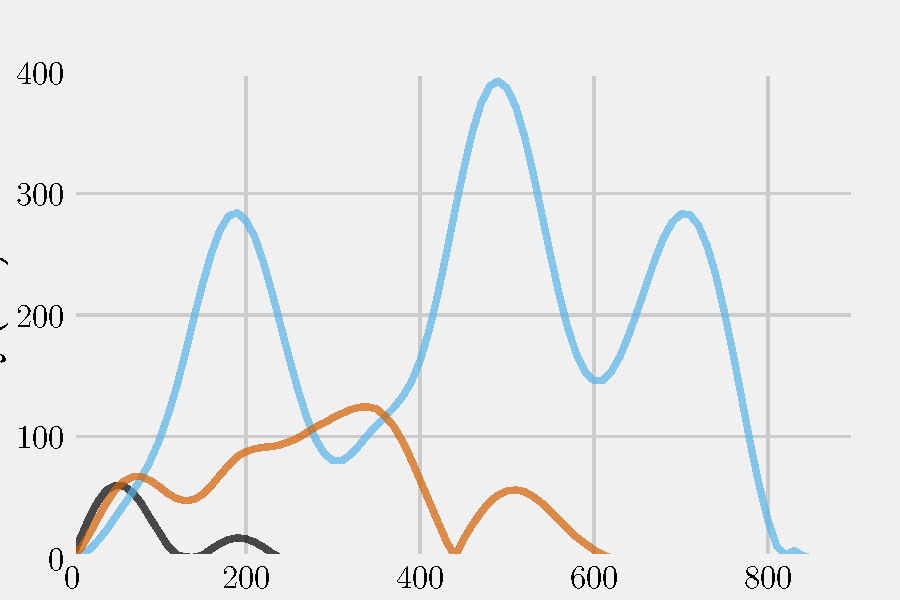
\includegraphics[width=\textwidth,keepaspectratio]{figures/gp_nn_training_smooth.pdf}
      \caption{ $b=60$ sec.}
      \label{fig:gp_nn_training_smooth}
  \end{subfigure}
  \begin{subfigure}[t]{.45\textwidth}
      \centering
      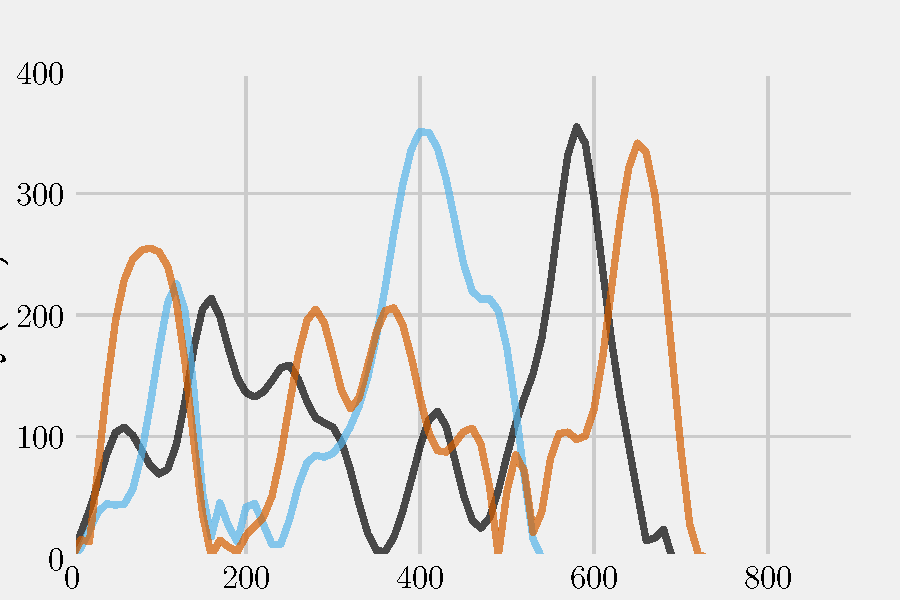
\includegraphics[width=\textwidth ,keepaspectratio]{figures/gp_nn_training_wiggly.pdf}
      \caption{ $b=30$ sec.}
      \label{fig:gp_nn_training_wiggly}
  \end{subfigure}
  \caption{Example draws from the Gaussian process generative model used to build the ANN emulator training set. \protect\ref{fig:gp_nn_training_smooth} shows that the drawn functions are smoother when using a bandwidth of 60 seconds compared to those shown in \protect\ref{fig:gp_nn_training_wiggly} when using a bandwidth of 30 seconds. The emulators train on functions drawn from both distributions. Note that the HRR curves also have a varying duration so that the emulators can learn to produce the results from FDS simulations with different simulation durations.} 
  \label{fig:gp_nn_training}
\end{figure}

A Python script was used to draw random HRR ramps, write them into FDS or CFAST input files, and then run the respective simulations. 

\clearpage
\subsection{Forward FDS emulators}
In this section, the design of the \textit{forward} emulators of FDS is described. For each thermocouple, an ANN is trained to map the time series vector $\dot{Q}(\boldsymbol{t}^\text{NN})$ to the corresponding temperature time series vector from an FDS simulation, $T_i(\boldsymbol{t}^\text{NN})$, where the index $i$ denotes the $ith$ thermocouple. Recall that $\boldsymbol{t}^\text{NN} = [0, 10, ..., 900]^T $. Note that FDS does note necessarily output a prediction at the times in $\boldsymbol{t}^\text{NN}$, so linear interpolation is used. For each ANN, the input layer and output layer both contain 91 nodes, which is equal to the length of $\boldsymbol{t}^\text{NN}$. There are four hidden layers, each with 128 \textit{perceptrons}. These are nodes that compute a weighted sum of their inputs and a bias, and then pass this sum through an activation function. The rectified linear activation function (ReLU) is used as the activation function. This function simply returns its input if the input is positive and returns zero otherwise.

The architecture of the ANNs is shown in Figure \ref{fig:neural_network_diagram} and the diagram of an individual perceptron is shown in Figure \ref{fig:perceptron_diagram}

\begin{figure}[htbp]
  \centering
  \begin{subfigure}[t]{.75\textwidth}
      \centering
      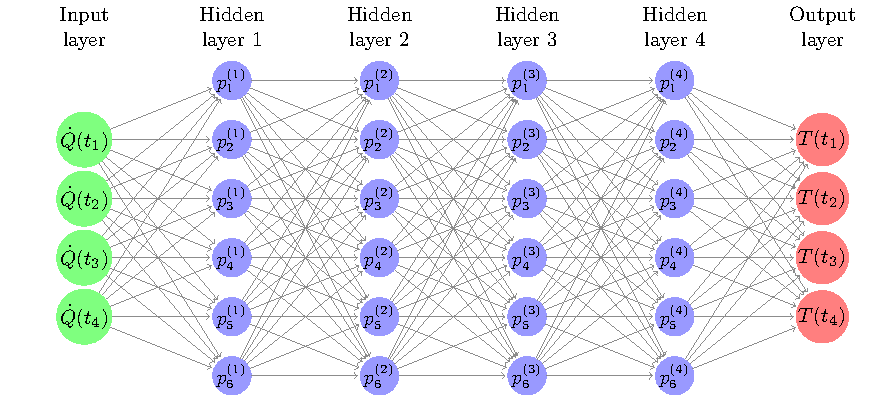
\includegraphics[width=\textwidth,keepaspectratio]{figures/neural_network_diagram.pdf}
      \caption{A simplified diagram of an ANN}
      \label{fig:neural_network_diagram}
  \end{subfigure}
  \begin{subfigure}[t]{.5\textwidth}
      \centering
      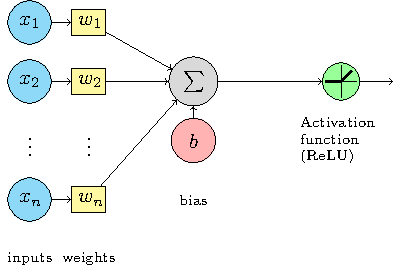
\includegraphics[width=\textwidth ,keepaspectratio]{figures/perceptron_diagram.pdf}
      \caption{A diagram of an individual perceptron}
      \label{fig:perceptron_diagram}
  \end{subfigure}
  \caption{\protect\ref{fig:neural_network_diagram} shows a simplified diagram of the neural network architecture used for each thermocouple response. In reality, the input layer and output layers each have 91 nodes as opposed to four, and each of the hidden layers has 128 perceptrons as opposed to six. The neural network is fully connected, meaning that each output of a given layer is an input to every perceptron in the next layer. \protect\ref{fig:perceptron_diagram} is a diagram showing the operation of an individual perceptron. All of the inputs to a given perceptron are weighted and then summed with an additional bias parameter. The result of this summation is sent through an activation function, which is the rectified linear activation function (ReLU) with the exception of the output layer, which simply outputs the sum.} 
  \label{fig:neural_network_drawings}
\end{figure}

Each perceptron in the first hidden layer has 92 parameters to learn (91 weights plus one bias) and all other perceptrons have 129 parameters to learn (128 weights plus one bias). This totals to 73,051 trainable parameters. The ANNs are constructed using the sequential method in the Python package Keras \cite{chollet2018keras}, which is built on top of TensorFlow. The parameters are trained using the Adam method \cite{kingma2014adam}, which is a stochastic optimization method. The batch size is set to 31, the validation split is  20\% of the data. Also, the authors found that the performance improved by dividing $\dot{Q}(t)$ by 200 kW and $\Delta T(t)$ by 200 $^oC$. This normalization makes it so that the inputs and outputs will generally vary on the order of one, which can lead to improved training \cite{sola1997importance}. 

The training process also leveraged transfer learning, which is the based on the idea that an agent can learn a task more efficiently if it has already been trained to perform a similar task. If transfer learning is not used, the weights and biases of the emulator ANNs are initialized with random values at the start of training. Instead, an ANN was first trained to predict the transient upper gas layer temperature in CFAST. A training set of 20,000 randomly generated CFAST cases was used for this initial training step. The weights and biases from this trained ANN are then used as the initial state for the ANN that is trained to predict the first FDS thermocouple. This process essentially transfers the knowledge of the simplified zone model physics of CFAST to the ANNs that learn the more complicated physics of FDS. Once the first FDS emulator is trained, its weights and biases are used to initialize each of the 16 remaining emulators. The transfer learning approach is depicted in the flow chart, Figure \ref{fig:transfer_learning_diagram}.


\begin{figure}[htb] \centering
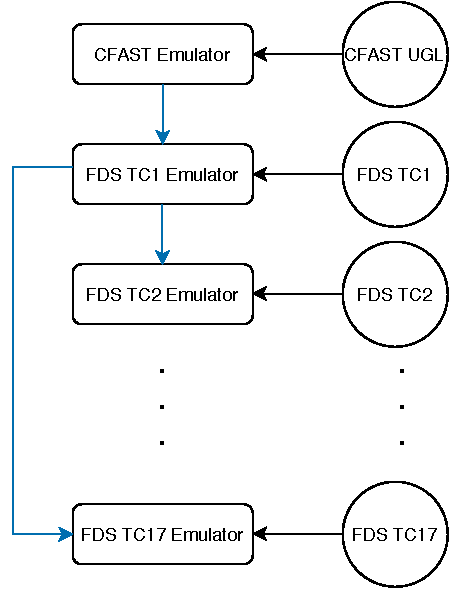
\includegraphics[width=.5\textwidth]{figures/transfer_learning_diagram.pdf}
\caption{A flow chart summarizing the transfer learning approach used during training. The circles represent outputs from compartment fire simulations. The rectangles represent emulator ANNs. The black arrows represent direct training and the blue arrows represent knowledge transfers. For example, the first emulator trains on examples of the transient CFAST UGL from a cold state. This knowledge is passed to the first FDS emulator, which then trains on the respective thermocouple in FDS. This knowledge is then transferred to all other FDS emulators.}
\label{fig:transfer_learning_diagram}
\end{figure}

In order to evaluate the effect of the this transfer learning procedure on training efficiency, 100 randomly generated FDS runs were set aside as a ``test set." An ANN emulator (for a single thermocouple) was then trained using a variable number of FDS cases ranging from 100 to 1900 cases. Once trained, the emulator made predictions on the 100 cases in the test set and the mean absolute error was calculated. This process was done twice- once with a ``cold start" ANN (with randomly initialized parameters) and again with an ANN that was initialized with the parameters from the trained CFAST ANN. Figure \ref{fig:transfer_learning} shows the effect of this initialization. It appears that the use of this transfer learning procedure dramatically reduces the required size of the FDS training set. 

\begin{figure}[htb] \centering
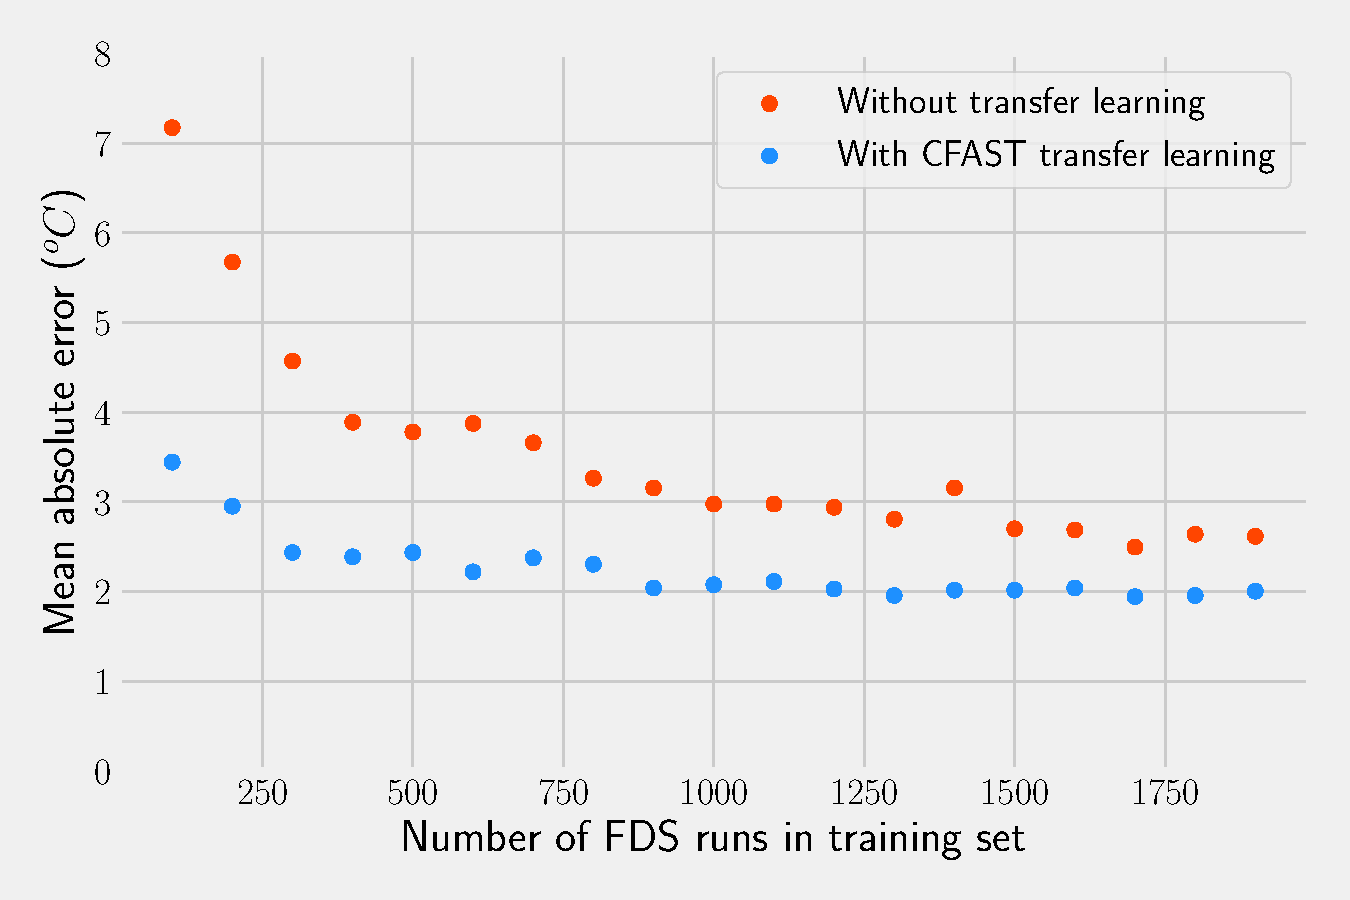
\includegraphics[width=.75\textwidth]{./figures/transfer_learning_effect.pdf}
\caption{A plot demonstrating the effect of pretraining an FDS emulator with the CFAST training set. If the FDS emulator is initialized with the weights and biases from a well trained CFAST UGL emulator, it can achieve lower error with a training set of 300 FDS runs than a ``cold start" emulator can with a training set of 1900 FDS runs.}
\label{fig:transfer_learning}
\end{figure}

For the results described in the rest of the paper, a training set of 1,000 FDS cases is used. Once trained, the emulators made predictions on the four HRR ramps that were used in the burner experiments shown in Figure \ref{fig:burner_ramps}. Keep in mind that none of these ramps are in the randomly generated training set. 

\begin{figure}[htbp]
  \centering
  \begin{subfigure}[t]{.45\textwidth}
      \centering
      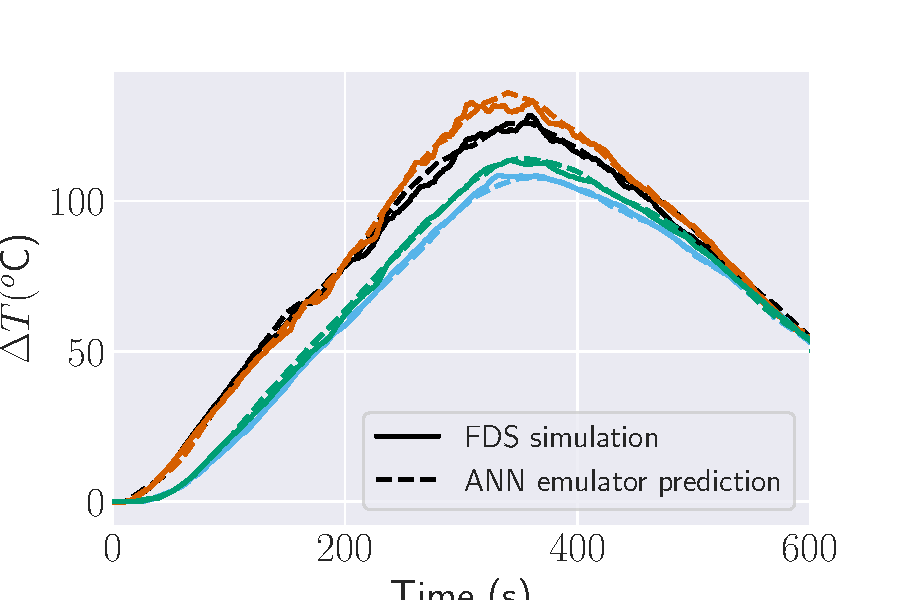
\includegraphics[width=\textwidth,keepaspectratio]{figures/forward_NN_examples.pdf}
      \caption{Example of emulator predictions compared to the corresponding FDS outputs}
      \label{fig:forward_NN_examples}
  \end{subfigure}
  \begin{subfigure}[t]{.45\textwidth}
      \centering
      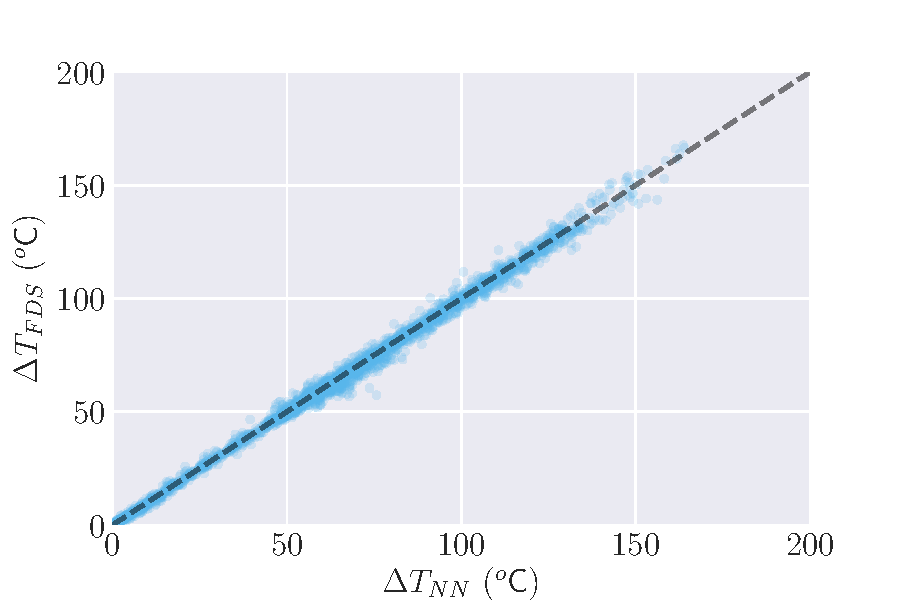
\includegraphics[width=\textwidth ,keepaspectratio]{figures/forward_error_scatter.pdf}
      \caption{Comparison of the FDS simulation results compared to the predicted output from the emulators across all four HRR ramps and all 17 thermocouples }
      \label{fig:forward_error_scatter}
  \end{subfigure}
  \caption{A comparison of the predictions of the ANN emulators compared to FDS simulations. \protect\ref{fig:forward_NN_examples} shows that the emulator outputs are typically smoother than the actual FDS outputs. \protect\ref{fig:forward_error_scatter} shows that the emulators successfully predict the FDS output for the four cases shown in Figure \protect\ref{fig:burner_ramps}. The mean absolute error across all thermocouples, all times, and all four HRR ramps is 1.6$^o$ C or 2.5\% of the average temperature.}
  \label{fig:forward_error}
\end{figure}

Figure \protect\ref{fig:forward_NN_examples} shows a typical output from the ANN emulators compared to an actual FDS simulation. The emulator predictions are typically smoother than the FDS outputs. This is likely due to the fact that the fluctuations in the FDS outputs are due to random turbulent effects, which are very difficult for the ANNs to learn. Overall the mean absolute error (MAE) of the emulator predictions compared to FDS is 1.6$^o$ C, indicating that they can accurately produce FDS outputs for new HRR curves. The emulators typically issue a full set of predictions (all 17 temperature time series) at a speed of about 80 iterations per second. On the same computer, it takes about 25 minutes to achieve the respective results from the FDS simulation, which equates to a speedup of over five orders of magnitude. 


\subsection{Inverse FDS emulators}
Another advantage of using ANN emulators to produce FDS outputs is that they can learn inverse mappings directly. The same ANN archeticure shown in Figure \ref{fig:neural_network_diagram} is used to produce 17 inverse emulators, except the quantities of the input and output layers are switched.  Each inverse emulator takes a temperature time series as an input and predicts the HRR ramp that would make FDS produce such an output for its respective thermocouple. This model can be especially useful because FDS does not natively have this functionality and iterative techniques are usually required. As before, the ANNs are first trained using the CFAST predicted upper gas layer. Using the FDS outputs for the four HRR curves shown in Figure \ref{fig:burner_ramps}, the inverse emulators each predicted the HRR ramp input that would cause FDS to produce the outputted transient temperature results. The results are shown in Figure \ref{fig:backward_examples}.

\begin{figure}[htbp]
  \centering
  \begin{subfigure}[t]{.45\textwidth}
      \centering
      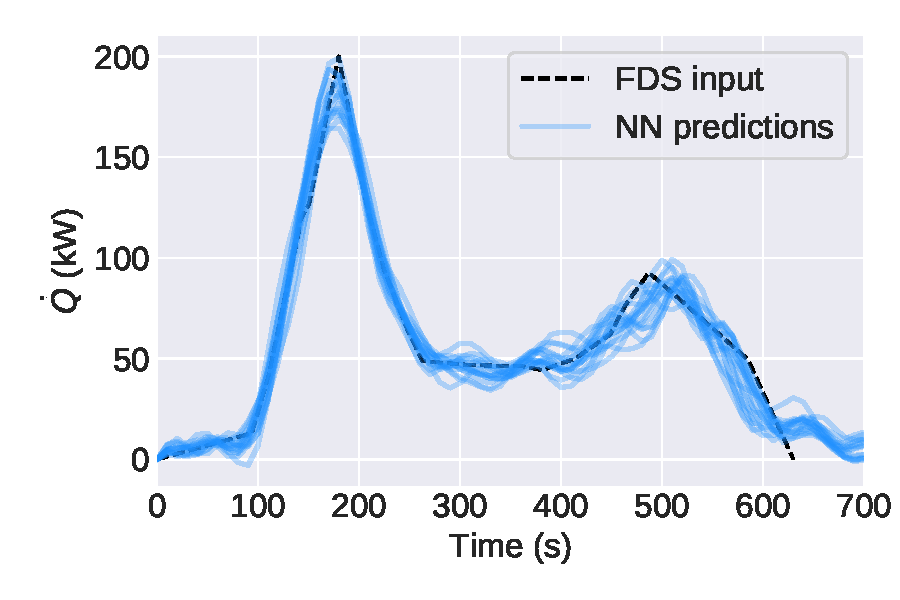
\includegraphics[width=\textwidth,keepaspectratio]{figures/backward_NN_examples.pdf}
      \caption{}
      \label{fig:backward_NN_examples}
  \end{subfigure}
  \begin{subfigure}[t]{.45\textwidth}
      \centering
      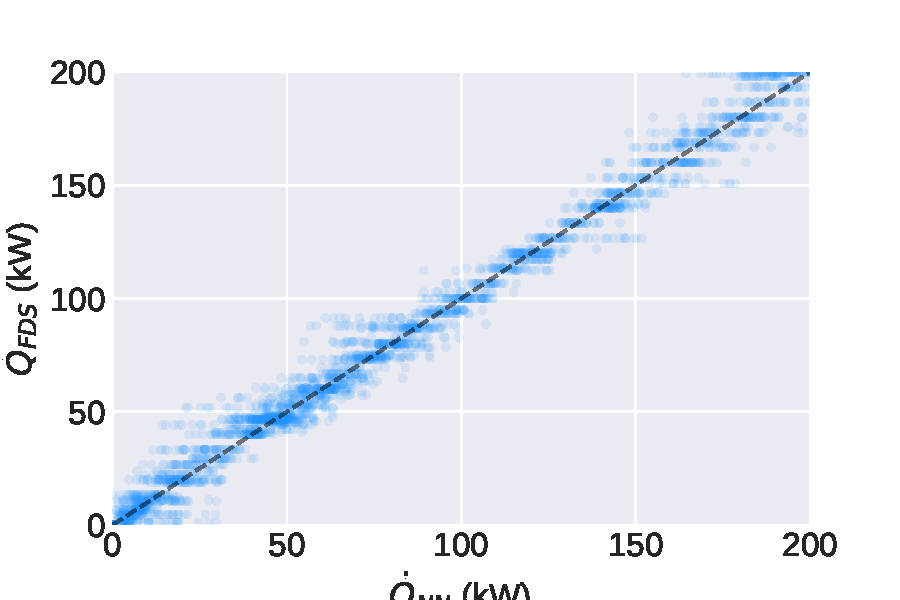
\includegraphics[width=\textwidth ,keepaspectratio]{figures/backward_error_scatter.pdf}
      \caption{}
      \label{fig:backward_error_scatter}
  \end{subfigure}
  \caption{Predictions of the inverse FDS emulators compared to the actual HRR inputs. In \protect\ref{fig:backward_NN_examples}, the dashed black line is the HRR input ramp for an FDS simulation. For each of the 17 thermocouple locations, an inverse ANN emulator uses the corresponding simulated temperature time series to predict the HRR ramp that would cause FDS to produce such an output. The 17 blue lines show the predicted HRR curves for the 17 different ANNs. \protect\ref{fig:backward_error_scatter} shows the actual HRR input compared to the predicted input for all 17 thermocouple locations, all times, and all four HRR ramps shown in Figure \protect\ref{fig:burner_ramps}. The MAE is 5.2 kW, or 6\% of the average HRR.} 
  \label{fig:backward_examples}
\end{figure}

Not surprisingly, the error as a percentage is greater for the inverse ANN emulators than for the forward ANN emulators. This may in part be due to the fact that the problem is ill-posed in the sense that there is no guarantee that a temperature output implies a unique HRR input. Nevertheless, the emulators generally reconstruct the HRR inputs accurately. It appears that they produce the most error when the slope of the HRR curve rapidly changes signs. This may be an artifact of the bandwidth selections in the Gaussian process generative model. Also, the emulators struggle to tell when the HRR goes to zero at the end of the ramp. This is likely due to the fact that the temperatures remain elevated for quite some time, even after the fire is extinguished. In experimental applications, this issue can may be mitigated by the fact that it is often visually clear when a fire is extinguished from video footage.

\section{Experimental applications}
This section explores the application of the ANN emulators of FDS for two experimental efforts- estimating the transient heat release rate of a burning item and inferring the radiative fraction of a burning fuel. All of these efforts depend on the ability of FDS to model the fire scenario accurately. Ideally, several controlled experiments with known HRR ramps could be performed initially in an experimental structure so that any errors in the FDS model could be corrected. However, this calibration process can be expensive and depends on equipment that some facilities do not have. As a result, an HRR inversion framework that does not require calibration experiments is presented first, followed by one that utilizes the calibration process to improve predictions. The framework for inferring the radiative fraction depends on quantifying the experimental error of the emulators, so calibration experiments are used for this procedure as well. 

\subsection{Heat release rate inversion}
The simplest approach for using the emulators to estimate a transient HRR is to pass the transient thermocouple measurements at the times in $\boldsymbol{t}^\text{NN}$ to the respective inverse ANN emulators. This results in 17 different predicted HRR curves (one for each thermocouple). In the absence of additional information, it is not clear whether any of these predictions is more credible than any of the others. As a result, a simple average of all of them is taken. 



\subsection{Bayesian inference of the radiative fraction}
\section{Conclusions}
\bibliographystyle{unsrtnat}
\bibliography{./references.bib}
\end{document}
